\chap{Adven: Momen Membangun Harapan}
\small

\section*{Pengertian Adven} 

Adven berasal dari bahasa Latin, \textit{adventus}, yang artinya kedatangan. Orang Katolik Perancis pada awalnya memakai kata \textit{adventus} untuk menamakan masa persiapan menyambut Hari Raya Epifani dimana para calon baptis dibaptis menjadi warga Gereja. Gereja Katolik kemudian memakai kata \textit{adventus} untuk menamakan masa persiapan perayaan Kelahiran Yesus Kristus, yaitu Hari Raya Natal. Masa Adven berlangsung selama 4 minggu, dimulai hari minggu dan biasanya setelah tanggal 26 November. Masa Adven mempunyai 2 tujuan utama, yaitu

\begin{enumerate}[itemsep=0ex]
\item mengarahkan hati, supaya dengan penuh harapan kita menantikan kedatangan Tuhan Yesus yang kedua pada akhir zaman.
\item menyiapkan Hari Natal, memperingati kedatangan Tuhan Yesus yang pertama dulu, di Betlehem, dengan kata lain mempersiapkan kedatangan Yesus Kristus secara Sakramental pada hari Natal.
\end{enumerate}

Katekismus Gereja Katolik menekankan makna ganda ``kedatangan'' ini: ``Dalam perayaan liturgi Adven, Gereja menyongsong kedatangan Mesias; dengan demikian umat beriman mengambil bagian dalam persiapan yang lama menjelang kedatangan pertama Penebus dan membaharui di dalamnya kerinduan akan kedatangan-Nya yang kedua.'' Jadi makna adven untuk kita: bersiap-siap dan berjaga-jaga setiap saat dalam menantikan kedatangan Tuhan Yesus. Hakikat adven adalah persiapan diri. Persiapan diri yang seperti apakah itu, yaitu tindakan yang selalu berjaga-jaga (awareness), dan menyiapkan hati, dengan
\textbf{bertobat,
berdoa,} dan \textbf{
berbuat amal kasih
}

Oleh sebab itu, di satu pihak, umat beriman merefleksikan kembali dan didorong untuk merayakan kedatangan Kristus yang pertama ke dalam dunia ini. Kita merenungkan kembali misteri inkarnasi yang agung ketika Kristus merendahkan diri, mengambil rupa manusia, dan masuk dalam dimensi ruang dan waktu guna membebaskan kita dari dosa. Di lain pihak, kita  ingat dalam Syahadat bahwa Kristus akan datang kembali untuk mengadili orang yang hidup dan mati dan kita harus siap untuk bertemu dengannya. 

Adventus ini pada hakikatnya adalah seperti dalam injil, tentang perumpamaan dalam injil Matius, tentang 5 orang gadis bodoh dan 5 gadis pandai. Gadis-gadis pandai yang selain membawa pelitanya, mereka juga membawa bekal berupa minyak. Karena kita tidak tahu, akan hari maupun saatnya kan tiba. Jadi di masa adven inilah kita harus seperti gadis-gadis yang membawa bekal minyak. 

Kita memang harus selalu siap secara batiniah dalam menyambut kedatangan/kelahiran penebus kita. Apabila di dalam Injil membahasakan persiapan tersebut sebagai ``bekal'' minyak lentera yang penuh, nah, di dalam kehidupan kita secara nyata, ''bekal'' tersebut adalah: persiapan kita, dalam bentuk: bertobat, berdoa, dan beramal kasih. Nah, Masa persiapan ini berlangsung selama 4 minggu, kita biasa sebut sebagai 4 minggu persiapan. Meskipun minggu terakhir Adven pada umumnya terpotong dengan tibanya Hari Natal. Namun untuk adven kali ini, pas sekali, utuh, karena Hari Natal kita, jatuh di hari minggu. 

\section*{Lingkaran Adven}

\begin{wrapfigure}{l}{4cm}
\centering
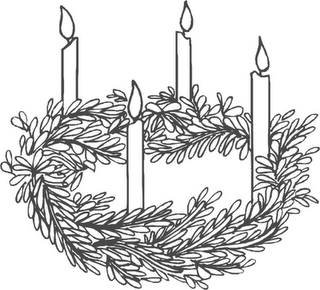
\includegraphics[scale=0.35]{gambar/advent4.png}
\end{wrapfigure}


\noindent{Pada masa adven, di gereja ada empat batang lilin, 3 yang berwarna ungu dan 1 berwarna merah muda. Dan diikat dengan lingkaran daun2 berwarna hijau. 
Warna ungu melambangkan Pertobatan, Adven adalah masa di mana kita mempersiapkan jiwa kita untuk menyambut kedatangan Kristus pada Hari Natal. Korona/lingkaran Adven, selalu dibuat dari daun-daun \textit{evergreen}. Dahan-dahan \textit{evergreen}, sama seperti namanya ``\textit{ever green}'' – senantiasa hijau, senantiasa hidup. \textit{Evergreen} melambangkan
\textbf{Pengharapan}, \textbf{Kehidupan}, itulah Kristus, yang mati namun hidup kembali untuk selamanya.
\textbf{Keabadian jiwa kita}. Kristus datang ke dunia untuk memberikan kehidupan yang tanpa akhir bagi kita.}

Tampak tersembul di antara daun-daun \textit{evergreen} yang hijau adalah buah-buah \textit{berry} warna merah. Buah-buah itu serupa tetesan-tetesan darah, lambang darah yang dicurahkan oleh Kristus demi umat manusia. Buah merah itu mengingatkan kita bahwa Kristus datang ke dunia untuk wafat bagi kita dan dengan demikian menebus kita. Oleh karena Darah-Nya yang tercurah itu, kita beroleh hidup yang kekal. Empat batang lilin diletakkan sekeliling Lingkaran Adven, tiga lilin berwarna ungu dan yang lain berwarna merah muda. Lilin-lilin itu melambangkan keempat minggu dalam Masa Adven, yaitu masa persiapan kita menyambut Natal. Setiap hari, dalam bacaan Liturgi Perjanjian Lama dikisahkan tentang penantian bangsa Yahudi akan datangnya Sang Mesias, sementara dalam Perjanjian Baru mulai diperkenalkan tokoh-tokoh yang berperan dalam Kisah Natal. Pada awal Masa Adven, sebatang lilin dinyalakan, kemudian setiap minggu berikutnya lilin lain mulai dinyalakan. Seiring dengan bertambah terangnya Lingkaran Adven setiap minggu dengan bertambah banyaknya lilin yang dinyalakan, kita pun diingatkan bahwa kelahiran Sang Terang Dunia semakin dekat. Semoga jiwa kita juga semakin menyala dalam kasih kepada Bayi Yesus. Warna-warni keempat lilin juga memiliki makna tersendiri. Lilin ungu sebagai lambang pertobatan. Lilin merah muda dinyalakan pada Hari Minggu Adven III yang disebut Minggu ``Gaudete''. ``Gaudete'' berasal dari bahasa Latin yang berarti ``sukacita'', melambangkan adanya sukacita di tengah masa pertobatan karena sukacita Natal hampir tiba. Warna merah muda dibuat dengan mencampurkan warna ungu dengan putih. Artinya, seolah-olah sukacita yang kita alami pada Hari Natal (yang dilambangkan dengan warna putih) sudah tidak tertahankan lagi dalam masa pertobatan ini (ungu) dan sedikit meledak dalam Masa Adven. Pada Hari Natal, keempat lilin tersebut digantikan dengan lilin-lilin putih – masa persiapan kita telah usai dan kita masuk dalam sukacita yang besar. Pada kaki setiap lilin, atau pada kaki Lingkaran Adven, ditempatkan sebuah mangkuk berwarna biru. Warna biru mengingatkan kita pada Bunda Maria, Bunda Allah, yang mengandung-Nya di dalam rahimnya serta melahirkan-Nya ke dunia pada hari Natal.

Lingkaran Adven diletakkan di tempat yang mencolok di gereja. Para keluarga memasang Lingkaran Adven yang lebih kecil di rumah mereka. Lingkaran Adven kecil ini mengingatkan mereka akan Lingkaran Adven di Gereja dan dengan demikian mengingatkan hubungan antara mereka dengan Gereja. Lilin dinyalakan pada saat makan bersama. Berdoa bersama sekeliling meja makan mengingatkan mereka akan meja perjamuan Tuhan di mana mereka berkumpul bersama setiap minggu untuk merayakan perjamuan Ekaristi - santapan dari Tuhan bagi jiwa kita. Jadi, nanti jika kita melihat atau memasang Lingkaran Adven, jangan menganggapnya sebagai hiasan yang indah saja. Ingatlah akan semua makna yang dilambangkannya, karena Lingkaran Adven hendak mengingatkan kita akan perlunya persiapan jiwa sehingga kita dapat sepenuhnya ambil bagian dalam sukacita besar Kelahiran Kristus, Putera Allah, yang telah memberikan Diri-Nya bagi kita agar kita beroleh hidup yang kekal.  


\section*{Minggu Adven}
Tiap-tiap minggu adven kita mengalami perhentian perjalanan batin kita. Seperti di dalam jalan salib, kita hening dan berdoa, mendengarkan pesan Allah. 

\subsection*{MINGGU ADVEN I}
Markus 13:33 , Yesus mengatakan kepada para muridnya: ``Hati-hatilah dan berjaga-jagalah! \ldots Kamu tidak tahu bilamanakah tuan rumah itu datang.'' Minggu I adven menjadi awal tahun liturgi gereja, Pesta Kristus Raja, selama 33 minggu biasa. 
Fokus: mempersiapkan umat untuk menyongsong kedatangan Yesus. 

\subsection*{MINGGU ADVEN II}
Markus 1:2b-3, ``Lihatlah, Aku menyuruh utusan-Ku mendahului Engkau, ia akan mempersiapkan jalan bagi-Mu; Ada suara orang yang berseru-seru di padang gurun: Persiapkanlah jalan untuk Tuhan, luruskanlah jalan bagi-Nya``

\subsection*{MINGGU ADVEN III}
Yohanes 1:26b, ``Di tengah-tengah kamu berdiri Dia yang tidak kamu kenal.''  Fokus : Yesus ada di tengah-tengah kita, namun kita tidak menyadarinya. Intinya, bahwa supaya kita mengetahui kehadirannya, kita harus benar-benar ``bersih'' dan peka, sehingga bahkan kita mampu mendengar Suara Tuhan, dan mengamalkannya. 

\subsection*{MINGGU ADVEN IV}
Lukas 1: 31 dan 38, ``Sesungguhnya engkau akan mengandung dan akanmelahirkan seorang anak laki-laki dan hendaklah engkau menamai Dia Yesus.'' 
``Sesungguhnya aku ini hamba Tuhan, terjadilah padaku menurut perkataanMu.'' 
Fokus : kita harus mengambil contoh seperti Bunda Maria yang suci, yang percaya dan yakin akan Allah. Sehingga, bahkan tidak tau maknanya pun Bunda Maria dengan pasrah dan tunduk akan kehendak Allah. Bagi kita, supaya kita suci dan layak untuk mengandung Yesus dlam diri kita, kitapun harus suci, yakin dan tunduk akan kehendak Allah akan kita. 

\section*{Warna Ungu: pertobatan}
Warna ungu disini berarti pertobatan, bukan seperti awam yang menganggap bahwa ungu itu berkabung. Pertobatan disini juga bertobat dengan penuh sukacita, karena kita sedang akan menjemput kedatanganNya yang kita nantikan. Membersihkan diri, memurnikan diri, supaya layak bertemu denganNya. Syarat untuk dapat diterima ke Kerajaan Sorga, simbol keselamatan dan kesejahteraan sejati yang abadi adalah Tobat. Tidak membawa apa-apa, harta benda, karir, gelar, prestasi  yang bisa membuat kita menjadi sombong, tinggi hati; kembali menjadi seperti bayi Kristus yang baru saja lahir. Adapun mengenai implikasi praktis dari pertobatan itu dinyatakan oleh Yohanes Pembaptis antara lain dengan menunjuk kepada perbuatan-perbuatan berikut, ``Barang siapa mempunyai dua helai baju, baiklah ia membaginya dengan yang tidak punya, dan barangsiapa mempunyai makanan, hendaklah ia berbuat juga demikian.'' 

Memang benar, bahwa Masa Adven adalah masa pertobatan. Kalau ada pesta-pesta Natal yang dilakukan dengan penuh gemerlap itu, selain mengacaukan persiapan menyongsong kelahiran Yesus, juga menggeser makna persiapan Natal yang sesungguhnya. Perayaan Natal yang dilakukan di pusat-pusat perbelanjaan sejak awal Desember mencerminkan adanya kepentingan lain yang pemodal besar yang tak lebih dari komersialisasi perayaan-perayaan Natal dengan tujuan akhir menarik pembeli. Akhirnya, pesan natal yang seharusnya disampaikan menjadi kabur. Pesan yang ingin disampaikanNya adalah kerendahan hati dan sikap solider dengan umat manusia lainnya, terutama rakyat kecil. Kelahiran-Nya dengan cara yang tak lazim itu pun melambangkan suatu kritik sosial terhadap praktik kekuasaan maupun praktik keagamaan pada zamannya. Apa yang ditampilkan dalam kegemerlapan perayaan Natal di mana-mana sesungguhnya merupakan sesuatu yang kontradiktif. Dalam hal ini, Gereja tidak berperan sendirian. Keluarga sebagai basis terkecil Gereja harus menanamkan kesadaran terhadap anggota keluarga untuk tidak terseret bisnis komersial pesta-pesta keagamaan. Anak muda perlu diingatkan bahwa materi bukan inti dari perayaan Natal, sebaliknya menjadi latihan yang menyegarkan bagi kesadaran, motivasi, untuk menciptakan perdamaian. Kalau Gereja tidak mampu menarik masyarakat untuk merenungi makna Natal itu, akibatnya pusat-pusat perbelanjaan yang akan lebih menarik masyarakat. Pesta keagamaan, merupakan pesta kerohanian. Sudah saatnya masing-masing pribadi memeriksa rohani kita sendiri dan motivasi diri. Tetapi, hal ini, dengan perayaan yang gemerlap ini, diserobot oleh materi. Kesadaran baru ini, akan memunculkan keinginan berkorban untuk orang yang berkesusahan melalui bantuan-bantuan yang nyata. Kesadaran itu harus dibangun dari lingkungan anak-anak, membangkitkan kesadaran kepada anak-anak agar lebih menghayati makna Natal, ketimbang pestanya. Yang penting perayaan Natal secara ESENSIAL daripada SENSASIONAL. 

Di satu sisi, di dalam keluarga dan masyarakat, sering mengikuti perayaan natal, pohon natal, pesta penyalaan lilin, yang membutuhkan biaya yang besar. Namun disisi yang lain, anak2 kita sudah melakukan amal kasih kepada sesama dengan mengumpulkan baju-baju dan mainan2 bekas untuk disumbangkan kepada saudara-saudara yang kurang beruntung.

Dalam Masa Adven ini, adalah KESEMPATAN untuk melihat kembali, \textit{flashback}, meninjau kembali apa yang sudah kita lakukan di masa lampau. Yang buruk ditinggalkan, dan yang baik ditingkatkan, untuk menuju hidup yang lebih baik dalam namaNya. Kemudian, yang saya lakukan yang lain, mengurangi makanan, supaya lebih memaknakan mati raga, dan berbagi rejeki pada yang kurang beruntung. Di lain pihak, pada saat mati raga itu, mendapatkan makna, bahwa doa bukan saja sebagai kegiatan rutin, namun lebih kepada KEBUTUHAN. Dengan mengurangi makanan, saya menjadi lebih peka terhadap dunia sekitar, bahwa dunia sedang banyak masalah, dan lain lain. 

\sumber{Narasumber Sr. Yohanika, MASF dan Bapak Gabriel Wujon} 
\normalsize